\documentclass[serif,mathserif,final]{beamer}
\mode<presentation>{\usetheme{Lankton}}


\usepackage{amsmath,amsfonts,amssymb,pxfonts,eulervm,xspace}
\usepackage{graphicx}
\usepackage{kerkis}
\graphicspath{{./figures/}}
%% coursera tells us the board will be 30in by 40in
\usepackage[orientation=landscape,size=custom,width=101,height=76,scale=2.3,debug]{beamerposter}

\newcommand{\mooculus}{\textsf{\textbf{MOOC}\upshape{ULUS}}}


\usebackgroundtemplate%
{%
    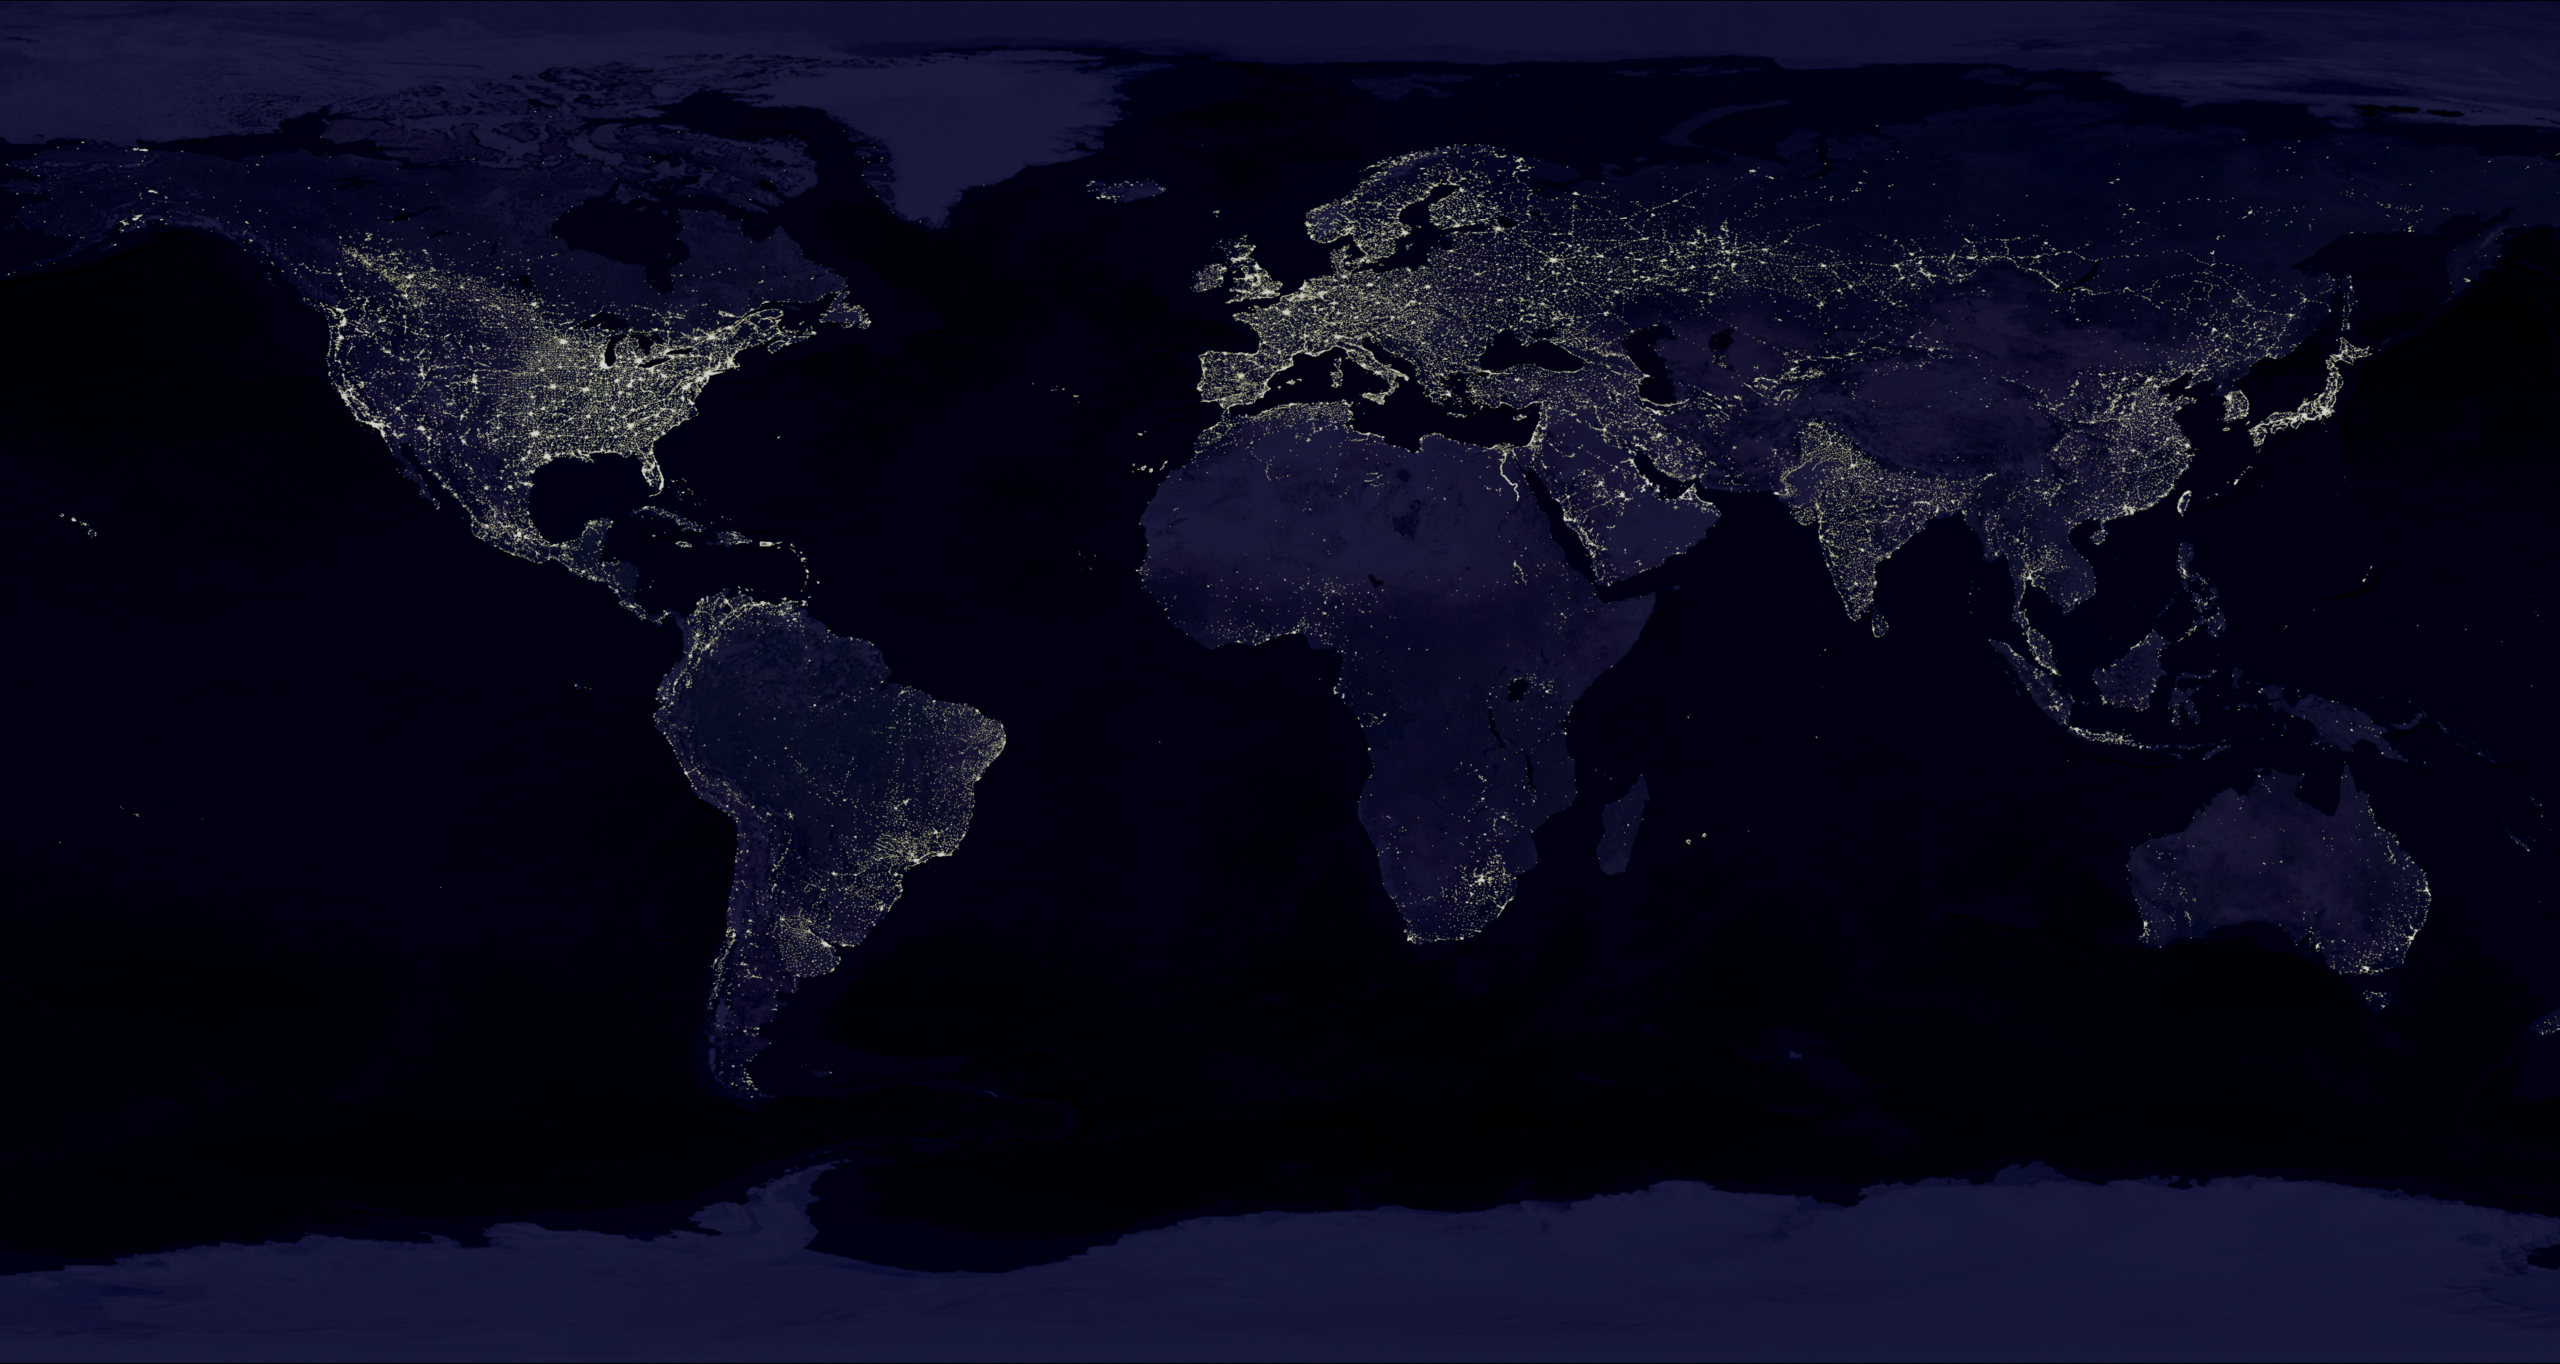
\includegraphics[width=\paperwidth,height=\paperheight]{Flat_earth_night.png}%
}

%-- Header and footer information ----------------------------------
\newcommand{\footleft}{\texttt{https://mooculus.osu.edu/}}
\newcommand{\footright}{
\includegraphics{qrcode}}%{shawn at shawn lankton dot com}
\title{\mdseries{Calculus\&}\mooculus}
\author{Tom Evans, Jim Fowler, Steve Gubkin, Bart Snapp}
\institute{The Ohio State University}
%-------------------------------------------------------------------


%-- Main Document --------------------------------------------------
\begin{document}
{
\usebackgroundtemplate{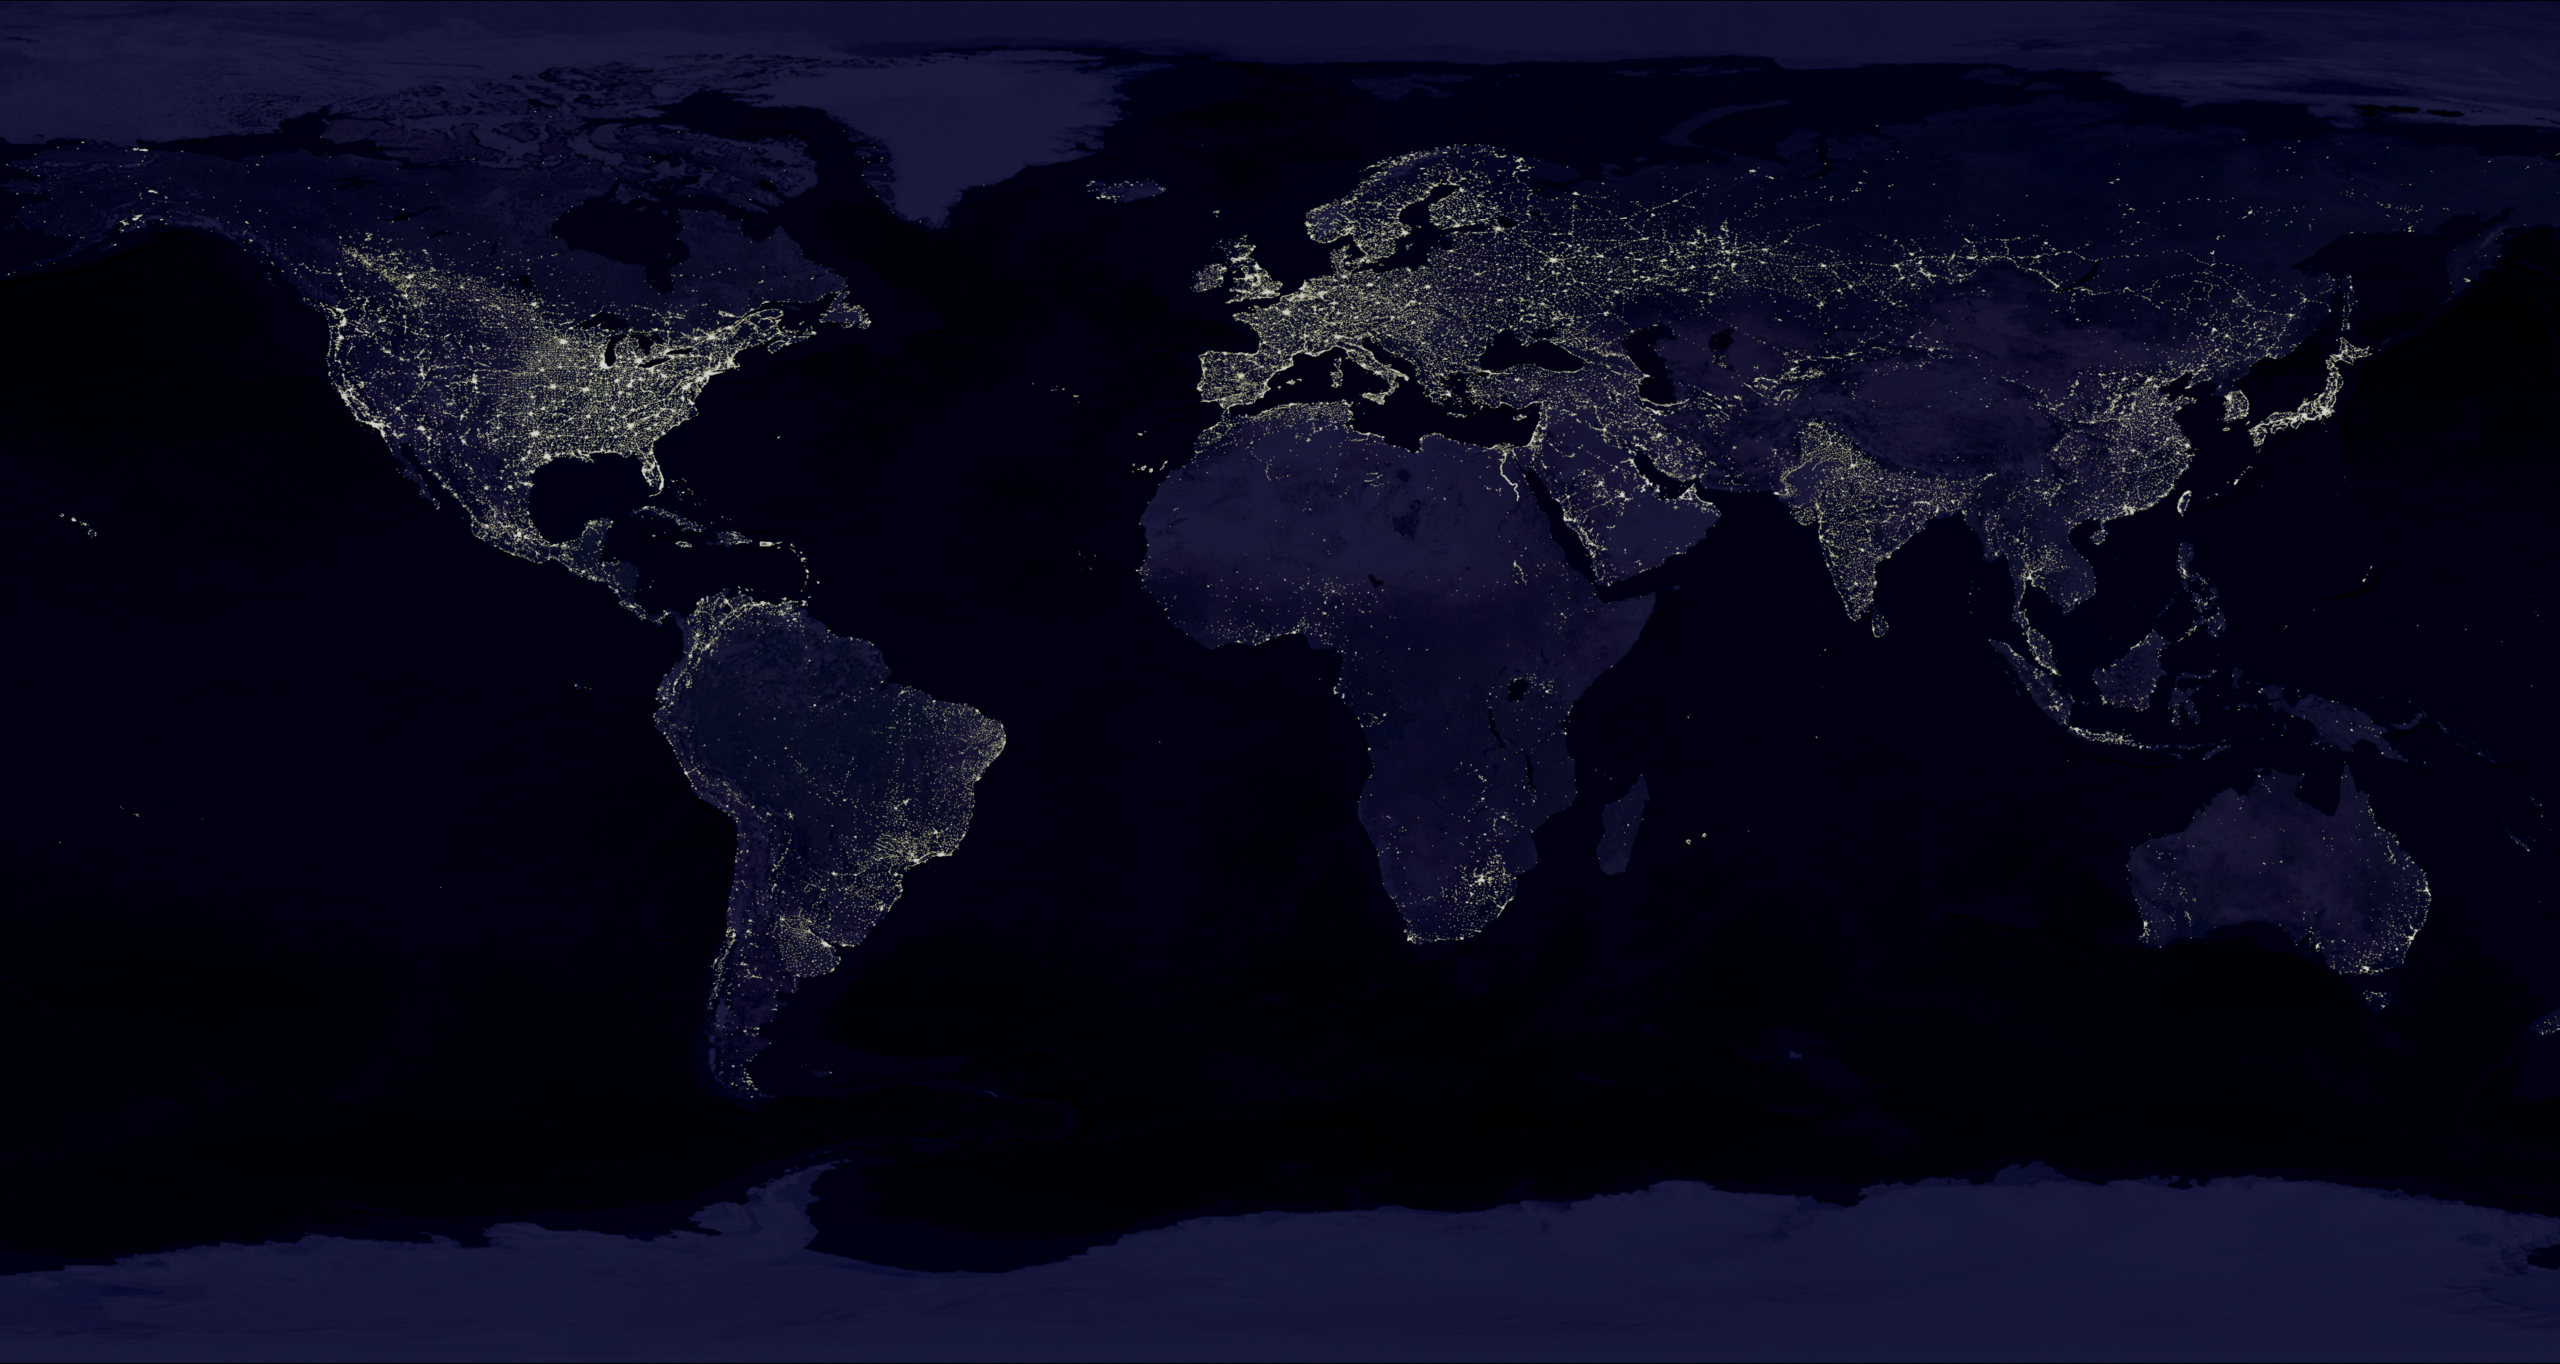
\includegraphics[height=\paperheight]{Flat_earth_night.png}}
\begin{frame}{}
  \begin{columns}[t]

    %-- Column 1 ---------------------------------------------------
    \begin{column}{0.32\linewidth}

      %-- Block 1-1
      \begin{block}{\rule{0pt}{1in}Coursera: Forums}
        \begin{figure}[htb]
          \centering
          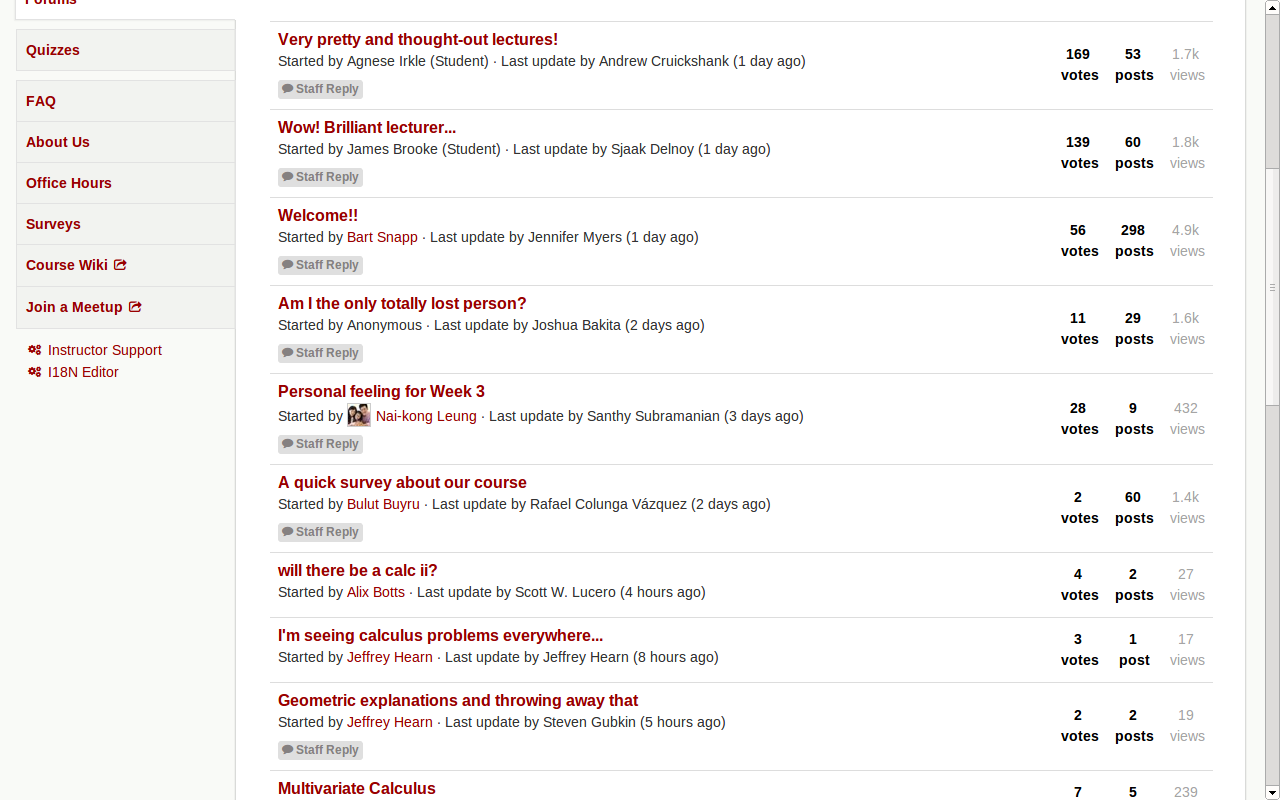
\includegraphics[width=.9\columnwidth]{forum}
        \end{figure}
        \end{block}

      \begin{block}{\rule{0pt}{1in}Coursera: Quizzes}
        \begin{figure}[htb]
          \centering
          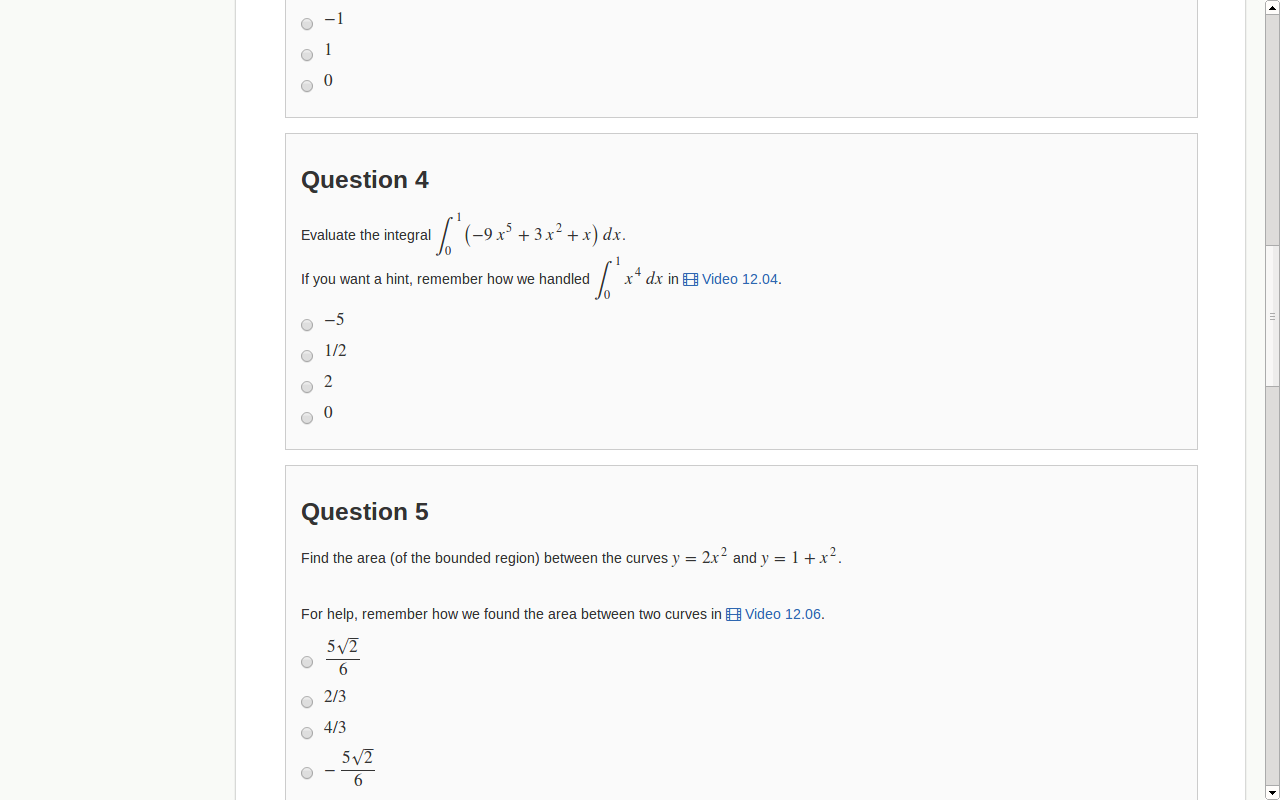
\includegraphics[width=.9\columnwidth]{quiz}
        \end{figure}
      \end{block}


    \end{column}%1

    %-- Column 2 ---------------------------------------------------
    \begin{column}{0.32\linewidth}

      %-- Block 2-1
      \begin{block}{\rule{0pt}{1in}\mooculus: Exercises}
        \begin{figure}[htb]
          \centering
          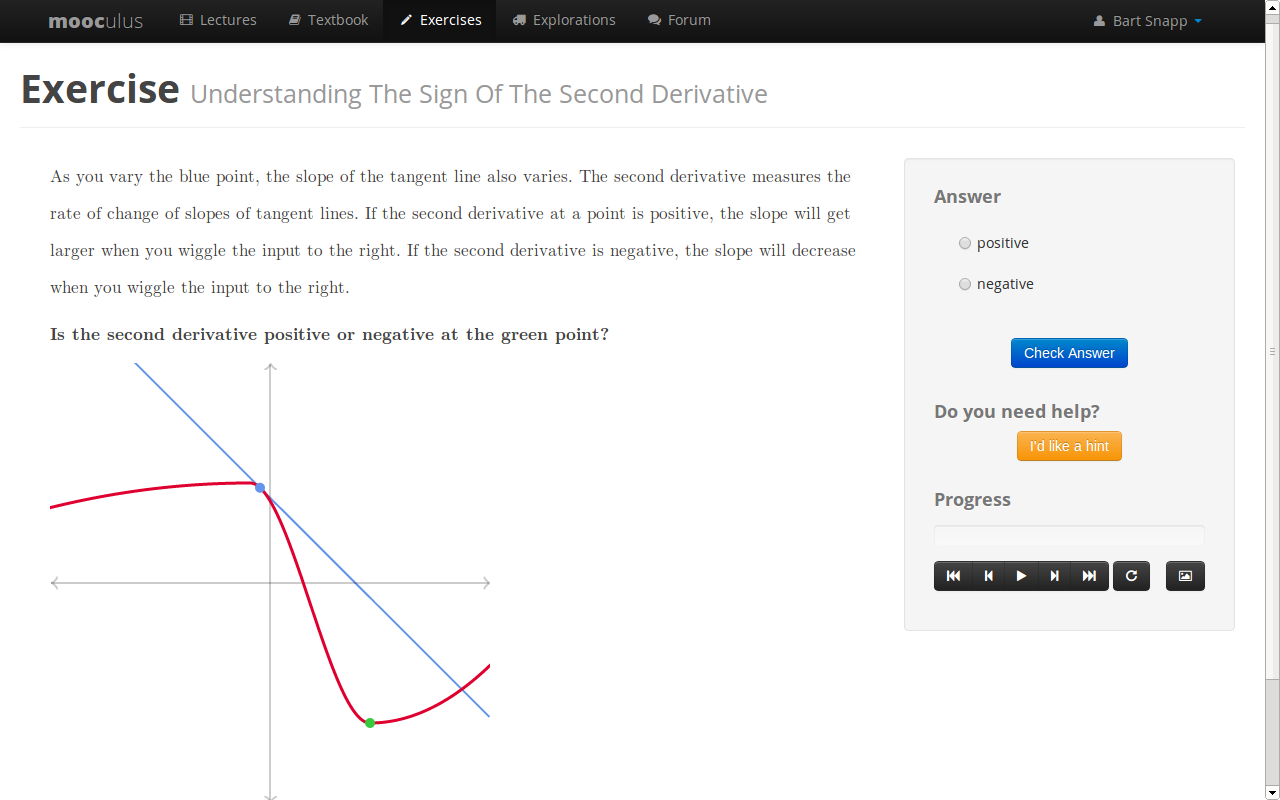
\includegraphics[width=.9\columnwidth]{exercise}
        \end{figure}
      \end{block}

      \begin{block}{\rule{0pt}{1in}\raisebox{.2\height}{\mooculus: Explorations}}
        \begin{figure}[htb]
          \centering
          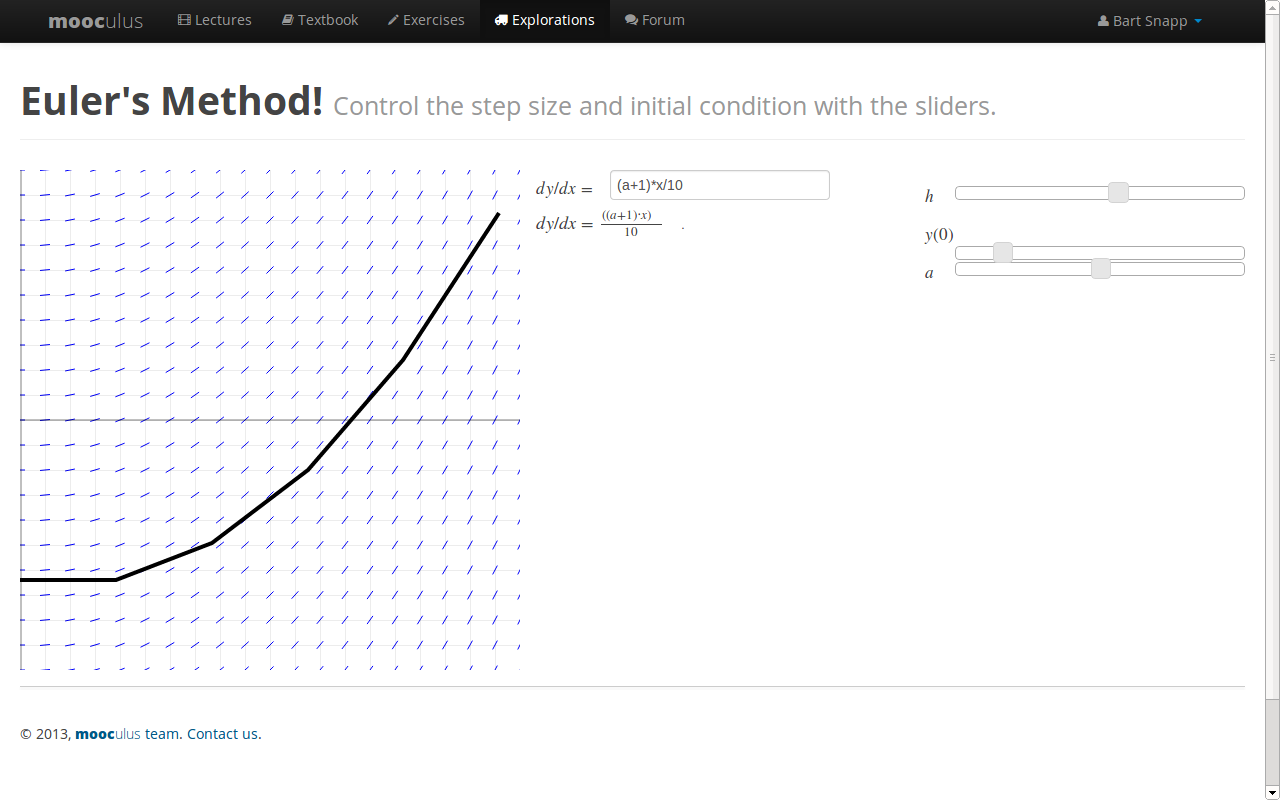
\includegraphics[width=.9\columnwidth]{exploration}
        \end{figure}
      \end{block}

    \end{column}%2

    %-- Column 3 ---------------------------------------------------
    \begin{column}{0.32\linewidth}

      %-- Block 3-1
      \begin{block}{\rule{0pt}{1in}Autocutter}
        \begin{figure}[htb]
        \centering
          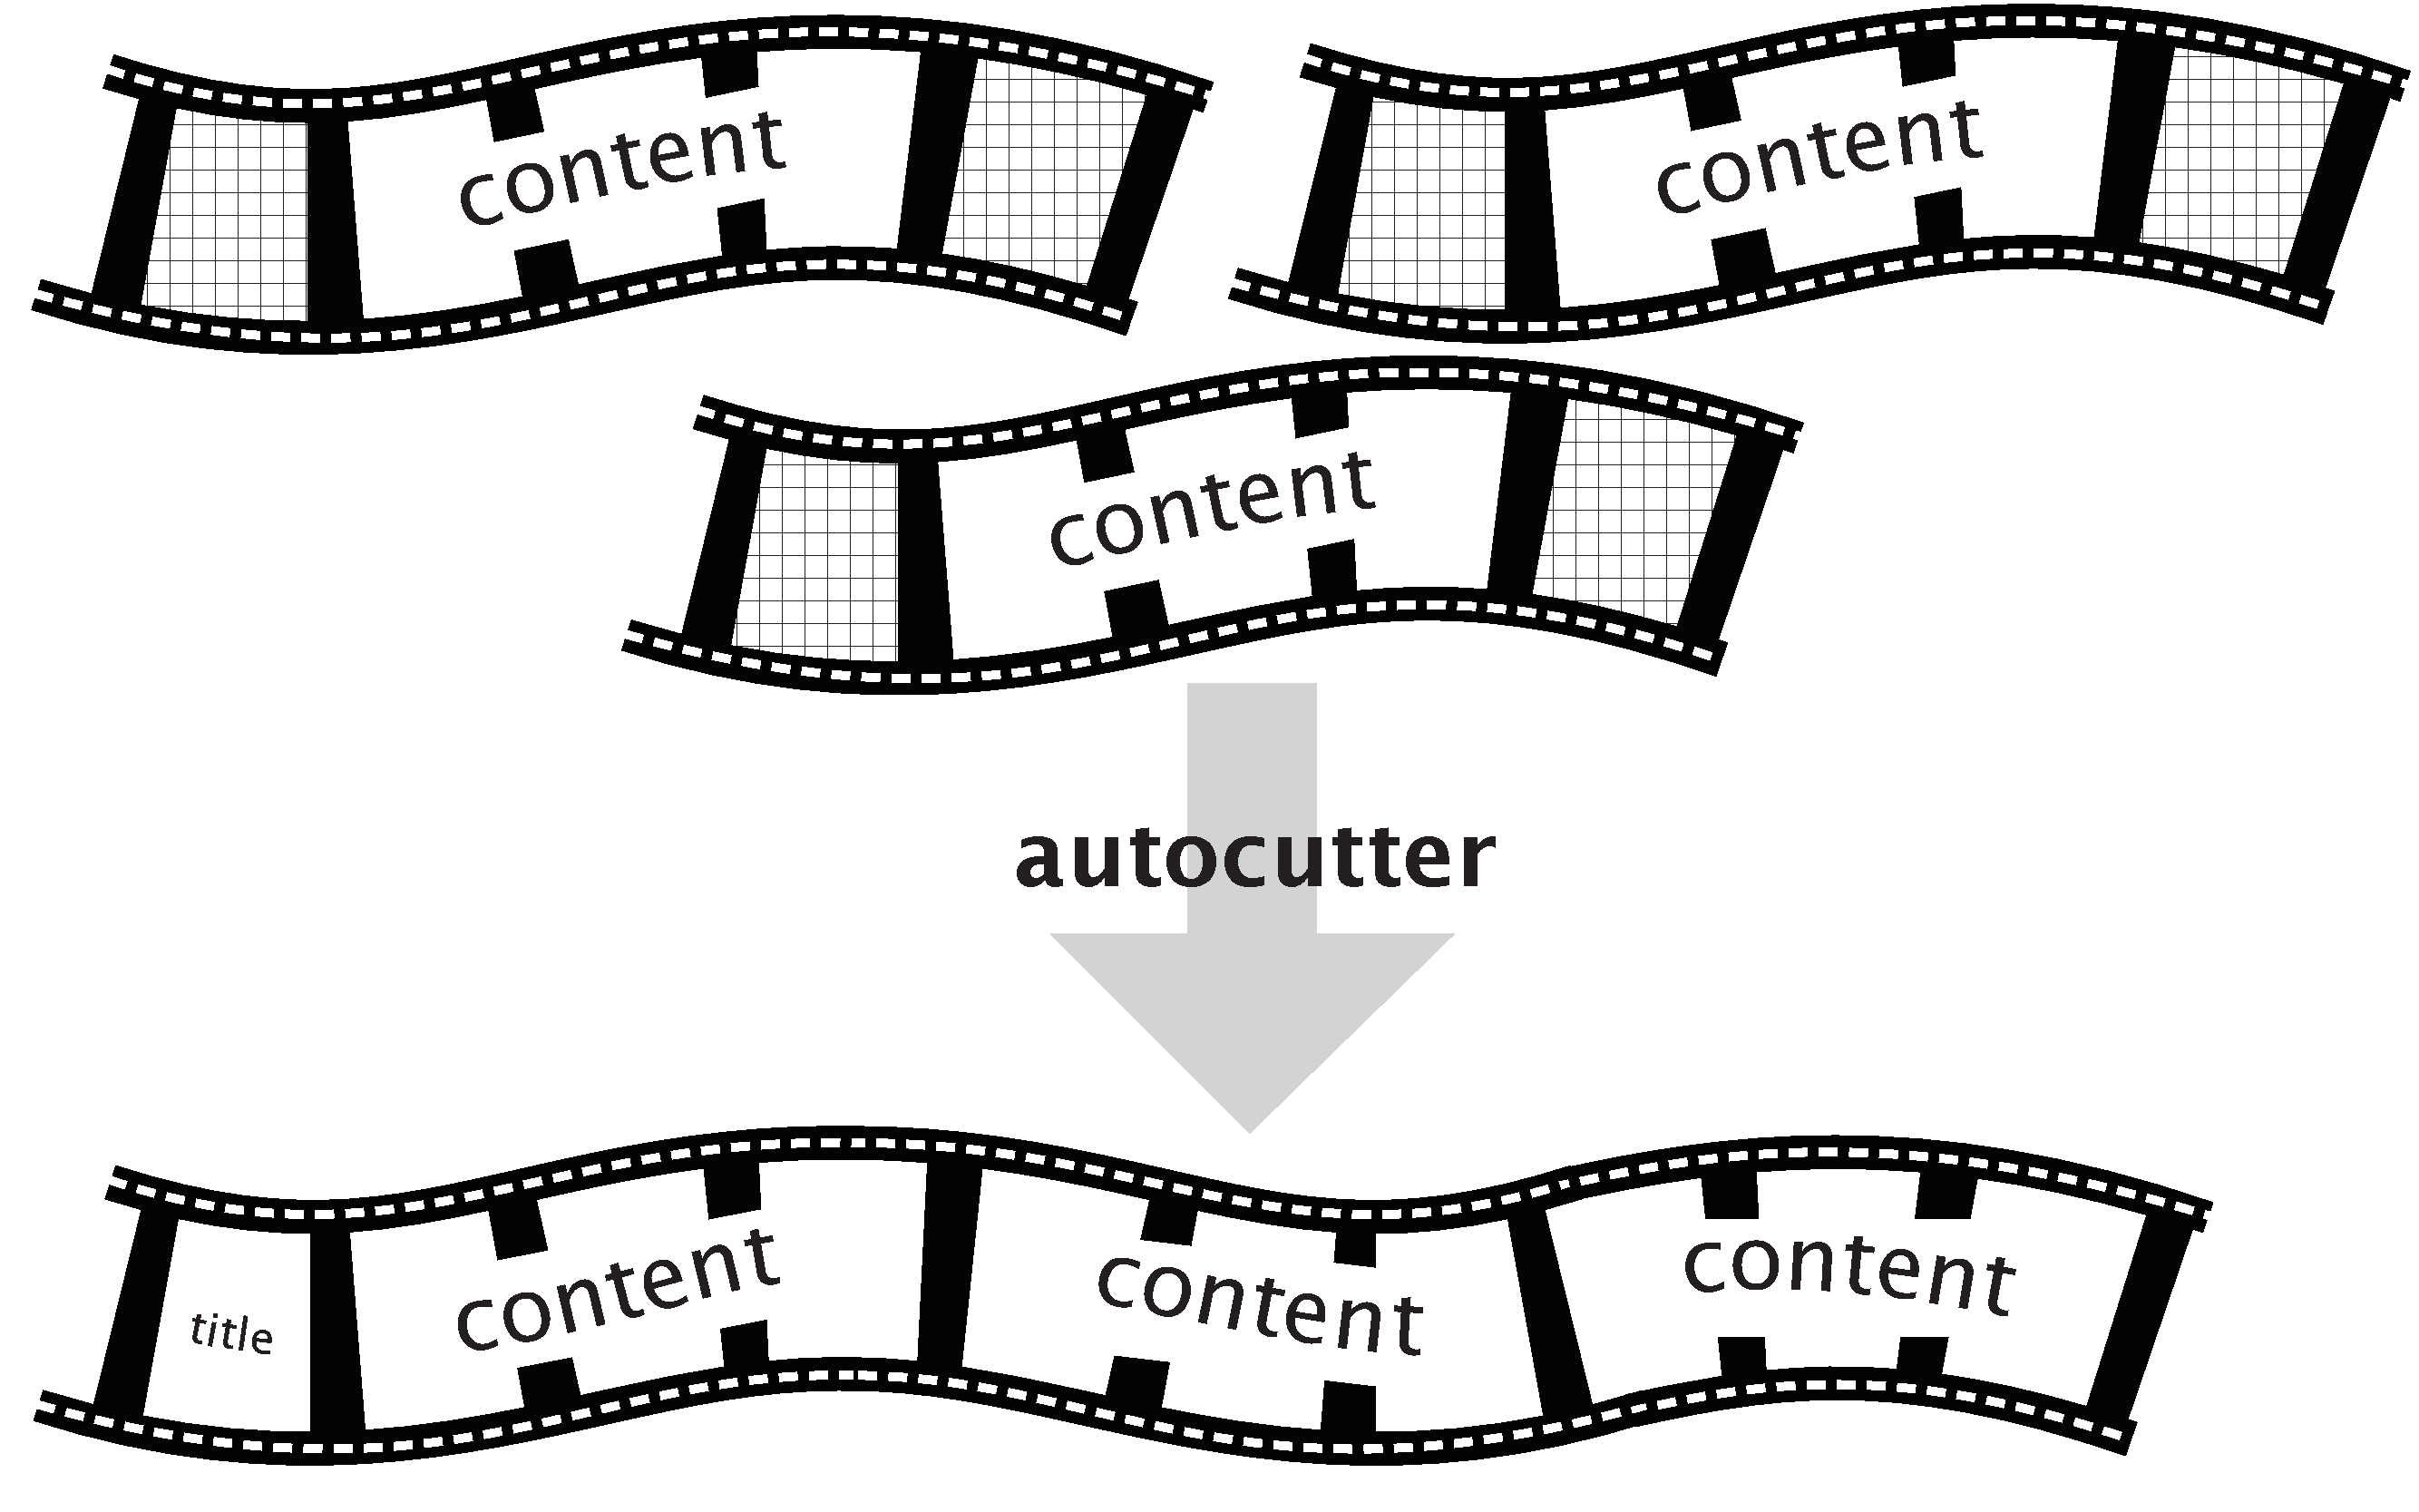
\includegraphics[width=.9\columnwidth]{autocutter}
        \end{figure}
      \end{block}

      %-- Block 3-2
      \begin{block}{\rule{0pt}{1in}\raisebox{.2\height}{Analytics}}
        \large
        \centering
        Over 35000 users\\

\vspace{2cm}

        Over 10 person-years\\

\vspace{2cm}
        Over 2 million correct answers

        \vspace{1.03in}
      \end{block}

    \end{column}%3
 
  \end{columns}
\end{frame}
}
\end{document}
